
% Default to the notebook output style

    


% Inherit from the specified cell style.




    
\documentclass[11pt]{article}

    
    
    \usepackage[T1]{fontenc}
    % Nicer default font (+ math font) than Computer Modern for most use cases
    \usepackage{mathpazo}

    % Basic figure setup, for now with no caption control since it's done
    % automatically by Pandoc (which extracts ![](path) syntax from Markdown).
    \usepackage{graphicx}
    % We will generate all images so they have a width \maxwidth. This means
    % that they will get their normal width if they fit onto the page, but
    % are scaled down if they would overflow the margins.
    \makeatletter
    \def\maxwidth{\ifdim\Gin@nat@width>\linewidth\linewidth
    \else\Gin@nat@width\fi}
    \makeatother
    \let\Oldincludegraphics\includegraphics
    % Set max figure width to be 80% of text width, for now hardcoded.
    \renewcommand{\includegraphics}[1]{\Oldincludegraphics[width=.8\maxwidth]{#1}}
    % Ensure that by default, figures have no caption (until we provide a
    % proper Figure object with a Caption API and a way to capture that
    % in the conversion process - todo).
    \usepackage{caption}
    \DeclareCaptionLabelFormat{nolabel}{}
    \captionsetup{labelformat=nolabel}

    \usepackage{adjustbox} % Used to constrain images to a maximum size 
    \usepackage{xcolor} % Allow colors to be defined
    \usepackage{enumerate} % Needed for markdown enumerations to work
    \usepackage{geometry} % Used to adjust the document margins
    \usepackage{amsmath} % Equations
    \usepackage{amssymb} % Equations
    \usepackage{textcomp} % defines textquotesingle
    % Hack from http://tex.stackexchange.com/a/47451/13684:
    \AtBeginDocument{%
        \def\PYZsq{\textquotesingle}% Upright quotes in Pygmentized code
    }
    \usepackage{upquote} % Upright quotes for verbatim code
    \usepackage{eurosym} % defines \euro
    \usepackage[mathletters]{ucs} % Extended unicode (utf-8) support
    \usepackage[utf8x]{inputenc} % Allow utf-8 characters in the tex document
    \usepackage{fancyvrb} % verbatim replacement that allows latex
    \usepackage{grffile} % extends the file name processing of package graphics 
                         % to support a larger range 
    % The hyperref package gives us a pdf with properly built
    % internal navigation ('pdf bookmarks' for the table of contents,
    % internal cross-reference links, web links for URLs, etc.)
    \usepackage{hyperref}
    \usepackage{longtable} % longtable support required by pandoc >1.10
    \usepackage{booktabs}  % table support for pandoc > 1.12.2
    \usepackage[inline]{enumitem} % IRkernel/repr support (it uses the enumerate* environment)
    \usepackage[normalem]{ulem} % ulem is needed to support strikethroughs (\sout)
                                % normalem makes italics be italics, not underlines
    

    
    
    % Colors for the hyperref package
    \definecolor{urlcolor}{rgb}{0,.145,.698}
    \definecolor{linkcolor}{rgb}{.71,0.21,0.01}
    \definecolor{citecolor}{rgb}{.12,.54,.11}

    % ANSI colors
    \definecolor{ansi-black}{HTML}{3E424D}
    \definecolor{ansi-black-intense}{HTML}{282C36}
    \definecolor{ansi-red}{HTML}{E75C58}
    \definecolor{ansi-red-intense}{HTML}{B22B31}
    \definecolor{ansi-green}{HTML}{00A250}
    \definecolor{ansi-green-intense}{HTML}{007427}
    \definecolor{ansi-yellow}{HTML}{DDB62B}
    \definecolor{ansi-yellow-intense}{HTML}{B27D12}
    \definecolor{ansi-blue}{HTML}{208FFB}
    \definecolor{ansi-blue-intense}{HTML}{0065CA}
    \definecolor{ansi-magenta}{HTML}{D160C4}
    \definecolor{ansi-magenta-intense}{HTML}{A03196}
    \definecolor{ansi-cyan}{HTML}{60C6C8}
    \definecolor{ansi-cyan-intense}{HTML}{258F8F}
    \definecolor{ansi-white}{HTML}{C5C1B4}
    \definecolor{ansi-white-intense}{HTML}{A1A6B2}

    % commands and environments needed by pandoc snippets
    % extracted from the output of `pandoc -s`
    \providecommand{\tightlist}{%
      \setlength{\itemsep}{0pt}\setlength{\parskip}{0pt}}
    \DefineVerbatimEnvironment{Highlighting}{Verbatim}{commandchars=\\\{\}}
    % Add ',fontsize=\small' for more characters per line
    \newenvironment{Shaded}{}{}
    \newcommand{\KeywordTok}[1]{\textcolor[rgb]{0.00,0.44,0.13}{\textbf{{#1}}}}
    \newcommand{\DataTypeTok}[1]{\textcolor[rgb]{0.56,0.13,0.00}{{#1}}}
    \newcommand{\DecValTok}[1]{\textcolor[rgb]{0.25,0.63,0.44}{{#1}}}
    \newcommand{\BaseNTok}[1]{\textcolor[rgb]{0.25,0.63,0.44}{{#1}}}
    \newcommand{\FloatTok}[1]{\textcolor[rgb]{0.25,0.63,0.44}{{#1}}}
    \newcommand{\CharTok}[1]{\textcolor[rgb]{0.25,0.44,0.63}{{#1}}}
    \newcommand{\StringTok}[1]{\textcolor[rgb]{0.25,0.44,0.63}{{#1}}}
    \newcommand{\CommentTok}[1]{\textcolor[rgb]{0.38,0.63,0.69}{\textit{{#1}}}}
    \newcommand{\OtherTok}[1]{\textcolor[rgb]{0.00,0.44,0.13}{{#1}}}
    \newcommand{\AlertTok}[1]{\textcolor[rgb]{1.00,0.00,0.00}{\textbf{{#1}}}}
    \newcommand{\FunctionTok}[1]{\textcolor[rgb]{0.02,0.16,0.49}{{#1}}}
    \newcommand{\RegionMarkerTok}[1]{{#1}}
    \newcommand{\ErrorTok}[1]{\textcolor[rgb]{1.00,0.00,0.00}{\textbf{{#1}}}}
    \newcommand{\NormalTok}[1]{{#1}}
    
    % Additional commands for more recent versions of Pandoc
    \newcommand{\ConstantTok}[1]{\textcolor[rgb]{0.53,0.00,0.00}{{#1}}}
    \newcommand{\SpecialCharTok}[1]{\textcolor[rgb]{0.25,0.44,0.63}{{#1}}}
    \newcommand{\VerbatimStringTok}[1]{\textcolor[rgb]{0.25,0.44,0.63}{{#1}}}
    \newcommand{\SpecialStringTok}[1]{\textcolor[rgb]{0.73,0.40,0.53}{{#1}}}
    \newcommand{\ImportTok}[1]{{#1}}
    \newcommand{\DocumentationTok}[1]{\textcolor[rgb]{0.73,0.13,0.13}{\textit{{#1}}}}
    \newcommand{\AnnotationTok}[1]{\textcolor[rgb]{0.38,0.63,0.69}{\textbf{\textit{{#1}}}}}
    \newcommand{\CommentVarTok}[1]{\textcolor[rgb]{0.38,0.63,0.69}{\textbf{\textit{{#1}}}}}
    \newcommand{\VariableTok}[1]{\textcolor[rgb]{0.10,0.09,0.49}{{#1}}}
    \newcommand{\ControlFlowTok}[1]{\textcolor[rgb]{0.00,0.44,0.13}{\textbf{{#1}}}}
    \newcommand{\OperatorTok}[1]{\textcolor[rgb]{0.40,0.40,0.40}{{#1}}}
    \newcommand{\BuiltInTok}[1]{{#1}}
    \newcommand{\ExtensionTok}[1]{{#1}}
    \newcommand{\PreprocessorTok}[1]{\textcolor[rgb]{0.74,0.48,0.00}{{#1}}}
    \newcommand{\AttributeTok}[1]{\textcolor[rgb]{0.49,0.56,0.16}{{#1}}}
    \newcommand{\InformationTok}[1]{\textcolor[rgb]{0.38,0.63,0.69}{\textbf{\textit{{#1}}}}}
    \newcommand{\WarningTok}[1]{\textcolor[rgb]{0.38,0.63,0.69}{\textbf{\textit{{#1}}}}}
    
    
    % Define a nice break command that doesn't care if a line doesn't already
    % exist.
    \def\br{\hspace*{\fill} \\* }
    % Math Jax compatability definitions
    \def\gt{>}
    \def\lt{<}
    % Document parameters
    \title{report}
    
    
    

    % Pygments definitions
    
\makeatletter
\def\PY@reset{\let\PY@it=\relax \let\PY@bf=\relax%
    \let\PY@ul=\relax \let\PY@tc=\relax%
    \let\PY@bc=\relax \let\PY@ff=\relax}
\def\PY@tok#1{\csname PY@tok@#1\endcsname}
\def\PY@toks#1+{\ifx\relax#1\empty\else%
    \PY@tok{#1}\expandafter\PY@toks\fi}
\def\PY@do#1{\PY@bc{\PY@tc{\PY@ul{%
    \PY@it{\PY@bf{\PY@ff{#1}}}}}}}
\def\PY#1#2{\PY@reset\PY@toks#1+\relax+\PY@do{#2}}

\expandafter\def\csname PY@tok@w\endcsname{\def\PY@tc##1{\textcolor[rgb]{0.73,0.73,0.73}{##1}}}
\expandafter\def\csname PY@tok@c\endcsname{\let\PY@it=\textit\def\PY@tc##1{\textcolor[rgb]{0.25,0.50,0.50}{##1}}}
\expandafter\def\csname PY@tok@cp\endcsname{\def\PY@tc##1{\textcolor[rgb]{0.74,0.48,0.00}{##1}}}
\expandafter\def\csname PY@tok@k\endcsname{\let\PY@bf=\textbf\def\PY@tc##1{\textcolor[rgb]{0.00,0.50,0.00}{##1}}}
\expandafter\def\csname PY@tok@kp\endcsname{\def\PY@tc##1{\textcolor[rgb]{0.00,0.50,0.00}{##1}}}
\expandafter\def\csname PY@tok@kt\endcsname{\def\PY@tc##1{\textcolor[rgb]{0.69,0.00,0.25}{##1}}}
\expandafter\def\csname PY@tok@o\endcsname{\def\PY@tc##1{\textcolor[rgb]{0.40,0.40,0.40}{##1}}}
\expandafter\def\csname PY@tok@ow\endcsname{\let\PY@bf=\textbf\def\PY@tc##1{\textcolor[rgb]{0.67,0.13,1.00}{##1}}}
\expandafter\def\csname PY@tok@nb\endcsname{\def\PY@tc##1{\textcolor[rgb]{0.00,0.50,0.00}{##1}}}
\expandafter\def\csname PY@tok@nf\endcsname{\def\PY@tc##1{\textcolor[rgb]{0.00,0.00,1.00}{##1}}}
\expandafter\def\csname PY@tok@nc\endcsname{\let\PY@bf=\textbf\def\PY@tc##1{\textcolor[rgb]{0.00,0.00,1.00}{##1}}}
\expandafter\def\csname PY@tok@nn\endcsname{\let\PY@bf=\textbf\def\PY@tc##1{\textcolor[rgb]{0.00,0.00,1.00}{##1}}}
\expandafter\def\csname PY@tok@ne\endcsname{\let\PY@bf=\textbf\def\PY@tc##1{\textcolor[rgb]{0.82,0.25,0.23}{##1}}}
\expandafter\def\csname PY@tok@nv\endcsname{\def\PY@tc##1{\textcolor[rgb]{0.10,0.09,0.49}{##1}}}
\expandafter\def\csname PY@tok@no\endcsname{\def\PY@tc##1{\textcolor[rgb]{0.53,0.00,0.00}{##1}}}
\expandafter\def\csname PY@tok@nl\endcsname{\def\PY@tc##1{\textcolor[rgb]{0.63,0.63,0.00}{##1}}}
\expandafter\def\csname PY@tok@ni\endcsname{\let\PY@bf=\textbf\def\PY@tc##1{\textcolor[rgb]{0.60,0.60,0.60}{##1}}}
\expandafter\def\csname PY@tok@na\endcsname{\def\PY@tc##1{\textcolor[rgb]{0.49,0.56,0.16}{##1}}}
\expandafter\def\csname PY@tok@nt\endcsname{\let\PY@bf=\textbf\def\PY@tc##1{\textcolor[rgb]{0.00,0.50,0.00}{##1}}}
\expandafter\def\csname PY@tok@nd\endcsname{\def\PY@tc##1{\textcolor[rgb]{0.67,0.13,1.00}{##1}}}
\expandafter\def\csname PY@tok@s\endcsname{\def\PY@tc##1{\textcolor[rgb]{0.73,0.13,0.13}{##1}}}
\expandafter\def\csname PY@tok@sd\endcsname{\let\PY@it=\textit\def\PY@tc##1{\textcolor[rgb]{0.73,0.13,0.13}{##1}}}
\expandafter\def\csname PY@tok@si\endcsname{\let\PY@bf=\textbf\def\PY@tc##1{\textcolor[rgb]{0.73,0.40,0.53}{##1}}}
\expandafter\def\csname PY@tok@se\endcsname{\let\PY@bf=\textbf\def\PY@tc##1{\textcolor[rgb]{0.73,0.40,0.13}{##1}}}
\expandafter\def\csname PY@tok@sr\endcsname{\def\PY@tc##1{\textcolor[rgb]{0.73,0.40,0.53}{##1}}}
\expandafter\def\csname PY@tok@ss\endcsname{\def\PY@tc##1{\textcolor[rgb]{0.10,0.09,0.49}{##1}}}
\expandafter\def\csname PY@tok@sx\endcsname{\def\PY@tc##1{\textcolor[rgb]{0.00,0.50,0.00}{##1}}}
\expandafter\def\csname PY@tok@m\endcsname{\def\PY@tc##1{\textcolor[rgb]{0.40,0.40,0.40}{##1}}}
\expandafter\def\csname PY@tok@gh\endcsname{\let\PY@bf=\textbf\def\PY@tc##1{\textcolor[rgb]{0.00,0.00,0.50}{##1}}}
\expandafter\def\csname PY@tok@gu\endcsname{\let\PY@bf=\textbf\def\PY@tc##1{\textcolor[rgb]{0.50,0.00,0.50}{##1}}}
\expandafter\def\csname PY@tok@gd\endcsname{\def\PY@tc##1{\textcolor[rgb]{0.63,0.00,0.00}{##1}}}
\expandafter\def\csname PY@tok@gi\endcsname{\def\PY@tc##1{\textcolor[rgb]{0.00,0.63,0.00}{##1}}}
\expandafter\def\csname PY@tok@gr\endcsname{\def\PY@tc##1{\textcolor[rgb]{1.00,0.00,0.00}{##1}}}
\expandafter\def\csname PY@tok@ge\endcsname{\let\PY@it=\textit}
\expandafter\def\csname PY@tok@gs\endcsname{\let\PY@bf=\textbf}
\expandafter\def\csname PY@tok@gp\endcsname{\let\PY@bf=\textbf\def\PY@tc##1{\textcolor[rgb]{0.00,0.00,0.50}{##1}}}
\expandafter\def\csname PY@tok@go\endcsname{\def\PY@tc##1{\textcolor[rgb]{0.53,0.53,0.53}{##1}}}
\expandafter\def\csname PY@tok@gt\endcsname{\def\PY@tc##1{\textcolor[rgb]{0.00,0.27,0.87}{##1}}}
\expandafter\def\csname PY@tok@err\endcsname{\def\PY@bc##1{\setlength{\fboxsep}{0pt}\fcolorbox[rgb]{1.00,0.00,0.00}{1,1,1}{\strut ##1}}}
\expandafter\def\csname PY@tok@kc\endcsname{\let\PY@bf=\textbf\def\PY@tc##1{\textcolor[rgb]{0.00,0.50,0.00}{##1}}}
\expandafter\def\csname PY@tok@kd\endcsname{\let\PY@bf=\textbf\def\PY@tc##1{\textcolor[rgb]{0.00,0.50,0.00}{##1}}}
\expandafter\def\csname PY@tok@kn\endcsname{\let\PY@bf=\textbf\def\PY@tc##1{\textcolor[rgb]{0.00,0.50,0.00}{##1}}}
\expandafter\def\csname PY@tok@kr\endcsname{\let\PY@bf=\textbf\def\PY@tc##1{\textcolor[rgb]{0.00,0.50,0.00}{##1}}}
\expandafter\def\csname PY@tok@bp\endcsname{\def\PY@tc##1{\textcolor[rgb]{0.00,0.50,0.00}{##1}}}
\expandafter\def\csname PY@tok@fm\endcsname{\def\PY@tc##1{\textcolor[rgb]{0.00,0.00,1.00}{##1}}}
\expandafter\def\csname PY@tok@vc\endcsname{\def\PY@tc##1{\textcolor[rgb]{0.10,0.09,0.49}{##1}}}
\expandafter\def\csname PY@tok@vg\endcsname{\def\PY@tc##1{\textcolor[rgb]{0.10,0.09,0.49}{##1}}}
\expandafter\def\csname PY@tok@vi\endcsname{\def\PY@tc##1{\textcolor[rgb]{0.10,0.09,0.49}{##1}}}
\expandafter\def\csname PY@tok@vm\endcsname{\def\PY@tc##1{\textcolor[rgb]{0.10,0.09,0.49}{##1}}}
\expandafter\def\csname PY@tok@sa\endcsname{\def\PY@tc##1{\textcolor[rgb]{0.73,0.13,0.13}{##1}}}
\expandafter\def\csname PY@tok@sb\endcsname{\def\PY@tc##1{\textcolor[rgb]{0.73,0.13,0.13}{##1}}}
\expandafter\def\csname PY@tok@sc\endcsname{\def\PY@tc##1{\textcolor[rgb]{0.73,0.13,0.13}{##1}}}
\expandafter\def\csname PY@tok@dl\endcsname{\def\PY@tc##1{\textcolor[rgb]{0.73,0.13,0.13}{##1}}}
\expandafter\def\csname PY@tok@s2\endcsname{\def\PY@tc##1{\textcolor[rgb]{0.73,0.13,0.13}{##1}}}
\expandafter\def\csname PY@tok@sh\endcsname{\def\PY@tc##1{\textcolor[rgb]{0.73,0.13,0.13}{##1}}}
\expandafter\def\csname PY@tok@s1\endcsname{\def\PY@tc##1{\textcolor[rgb]{0.73,0.13,0.13}{##1}}}
\expandafter\def\csname PY@tok@mb\endcsname{\def\PY@tc##1{\textcolor[rgb]{0.40,0.40,0.40}{##1}}}
\expandafter\def\csname PY@tok@mf\endcsname{\def\PY@tc##1{\textcolor[rgb]{0.40,0.40,0.40}{##1}}}
\expandafter\def\csname PY@tok@mh\endcsname{\def\PY@tc##1{\textcolor[rgb]{0.40,0.40,0.40}{##1}}}
\expandafter\def\csname PY@tok@mi\endcsname{\def\PY@tc##1{\textcolor[rgb]{0.40,0.40,0.40}{##1}}}
\expandafter\def\csname PY@tok@il\endcsname{\def\PY@tc##1{\textcolor[rgb]{0.40,0.40,0.40}{##1}}}
\expandafter\def\csname PY@tok@mo\endcsname{\def\PY@tc##1{\textcolor[rgb]{0.40,0.40,0.40}{##1}}}
\expandafter\def\csname PY@tok@ch\endcsname{\let\PY@it=\textit\def\PY@tc##1{\textcolor[rgb]{0.25,0.50,0.50}{##1}}}
\expandafter\def\csname PY@tok@cm\endcsname{\let\PY@it=\textit\def\PY@tc##1{\textcolor[rgb]{0.25,0.50,0.50}{##1}}}
\expandafter\def\csname PY@tok@cpf\endcsname{\let\PY@it=\textit\def\PY@tc##1{\textcolor[rgb]{0.25,0.50,0.50}{##1}}}
\expandafter\def\csname PY@tok@c1\endcsname{\let\PY@it=\textit\def\PY@tc##1{\textcolor[rgb]{0.25,0.50,0.50}{##1}}}
\expandafter\def\csname PY@tok@cs\endcsname{\let\PY@it=\textit\def\PY@tc##1{\textcolor[rgb]{0.25,0.50,0.50}{##1}}}

\def\PYZbs{\char`\\}
\def\PYZus{\char`\_}
\def\PYZob{\char`\{}
\def\PYZcb{\char`\}}
\def\PYZca{\char`\^}
\def\PYZam{\char`\&}
\def\PYZlt{\char`\<}
\def\PYZgt{\char`\>}
\def\PYZsh{\char`\#}
\def\PYZpc{\char`\%}
\def\PYZdl{\char`\$}
\def\PYZhy{\char`\-}
\def\PYZsq{\char`\'}
\def\PYZdq{\char`\"}
\def\PYZti{\char`\~}
% for compatibility with earlier versions
\def\PYZat{@}
\def\PYZlb{[}
\def\PYZrb{]}
\makeatother


    % Exact colors from NB
    \definecolor{incolor}{rgb}{0.0, 0.0, 0.5}
    \definecolor{outcolor}{rgb}{0.545, 0.0, 0.0}



    
    % Prevent overflowing lines due to hard-to-break entities
    \sloppy 
    % Setup hyperref package
    \hypersetup{
      breaklinks=true,  % so long urls are correctly broken across lines
      colorlinks=true,
      urlcolor=urlcolor,
      linkcolor=linkcolor,
      citecolor=citecolor,
      }
    % Slightly bigger margins than the latex defaults
    
    \geometry{verbose,tmargin=1in,bmargin=1in,lmargin=1in,rmargin=1in}
    
    

    \begin{document}
    
    
    \maketitle
    
    

    
    \section{MCMD Course Project 5}\label{mcmd-course-project-5}

\subsubsection{Molecular Dynamics Simulations of
Biomolecules}\label{molecular-dynamics-simulations-of-biomolecules}

By: Samuel Wiqvist

    \subsection{Introduction}\label{introduction}

In this short report, we will use the AMBER software to perform
molecular dynamics simulations for biomolecules. In particular, we will
run some of the AMBER' tutorials and report what we find.

The code used in this project can be found here:
https://github.com/SamuelWiqvist/compute\_MCMD/tree/master/hw\_week\_5

    \subsection{An introduction to molecular dynamics simulations with
AMBER}\label{an-introduction-to-molecular-dynamics-simulations-with-amber}

We decided to use LUNARC to run the tutorials to load the AMBER software
on LUNARC we used

\begin{verbatim}
ml load icc/2017.4.196-GCC-6.4.0-2.28
ml load OpenMPI/2.1.1
ml load Ambertools/18.10
\end{verbatim}

Furthermore, we loaded VMD with

\begin{verbatim}
module load vmd/1.9.2
\end{verbatim}

Finally to generate the plots we used Grace, which we loaded with

\begin{verbatim}
module spider grace/5.1.25
\end{verbatim}

In the tutorial use ran an AMBER MD sander simulation in three steps: we
first ran the minimization, then we heated the system, and finally, we
ran the production. To run these three simulations, we used the
following script

\begin{verbatim}
#!/bin/sh

# need this since I use a LU project
#SBATCH -A lu2018-2-22
#SBATCH -p lu

# use gpu nodes
#SBATCH -N 1
#SBATCH -n 1

# time consumption HH:MM:SS
#SBATCH -t 1:00:00

# name for script
#SBATCH -J amber_run

# controll job outputs
#SBATCH -o lunarc_outputs_amber_md%j.out
#SBATCH -e lunarc_outputs_amber_md%j.err

# notification
#SBATCH --mail-user=samuel.wiqvist@matstat.lu.se
#SBATCH --mail-type=ALL

# load modules
ml load  icc/2017.4.196-GCC-6.4.0-2.28
ml load OpenMPI/2.1.1
ml load Ambertools/18.10

# Run minimization
$AMBERHOME/bin/sander -O -i 01_Min.in -o 01_Min.out -p parm7 -c rst7 -r 01_Min.ncrst \
-inf 01_Min.mdinfo

# Run heating MD
$AMBERHOME/bin/sander -O -i 02_Heat.in -o 02_Heat.out -p parm7 -c 01_Min.ncrst \
-r 02_Heat.ncrst -x 02_Heat.nc -inf 02_Heat.mdinfo

# Run production MD
$AMBERHOME/bin/sander -O -i 03_Prod.in -o 03_Prod.out -p parm7 -c 02_Heat.ncrst \
-r 03_Prod.ncrst -x 03_Prod.nc -inf 03_Prod.info 
\end{verbatim}

The three simulations took 8.5 min to run on \texttt{LUNARC}, which is
somewhat faster than what the tutorial says the simulations should be,
according to the tutorial, the last simulation should take 19 min alone.

After running the simulations, the rest of the tutorial consisted of
running some visualizations using VMD and Grace. We managed to run all
visualizations without problems. As, and example, the temperature during
the simulation is plotted below

\begin{figure}
\centering
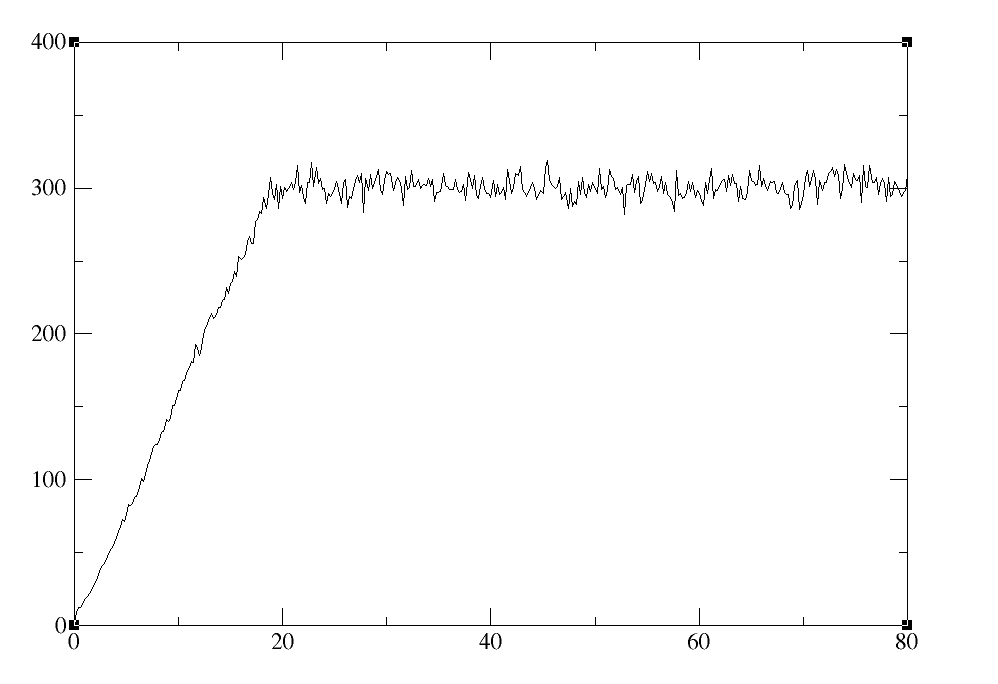
\includegraphics{Screenshot_temp_intro.png}
\caption{VMD layout}
\end{figure}

    \subsection{Using VMD with AMBER}\label{using-vmd-with-amber}

To run VMD on the LUNARC system, we first loaded VMD with the following
command

\begin{verbatim}
module load vmd/1.9.2
\end{verbatim}

\subsubsection{Section 1}\label{section-1}

After configuring the layout, we had following layou-t for VMD

\begin{figure}
\centering
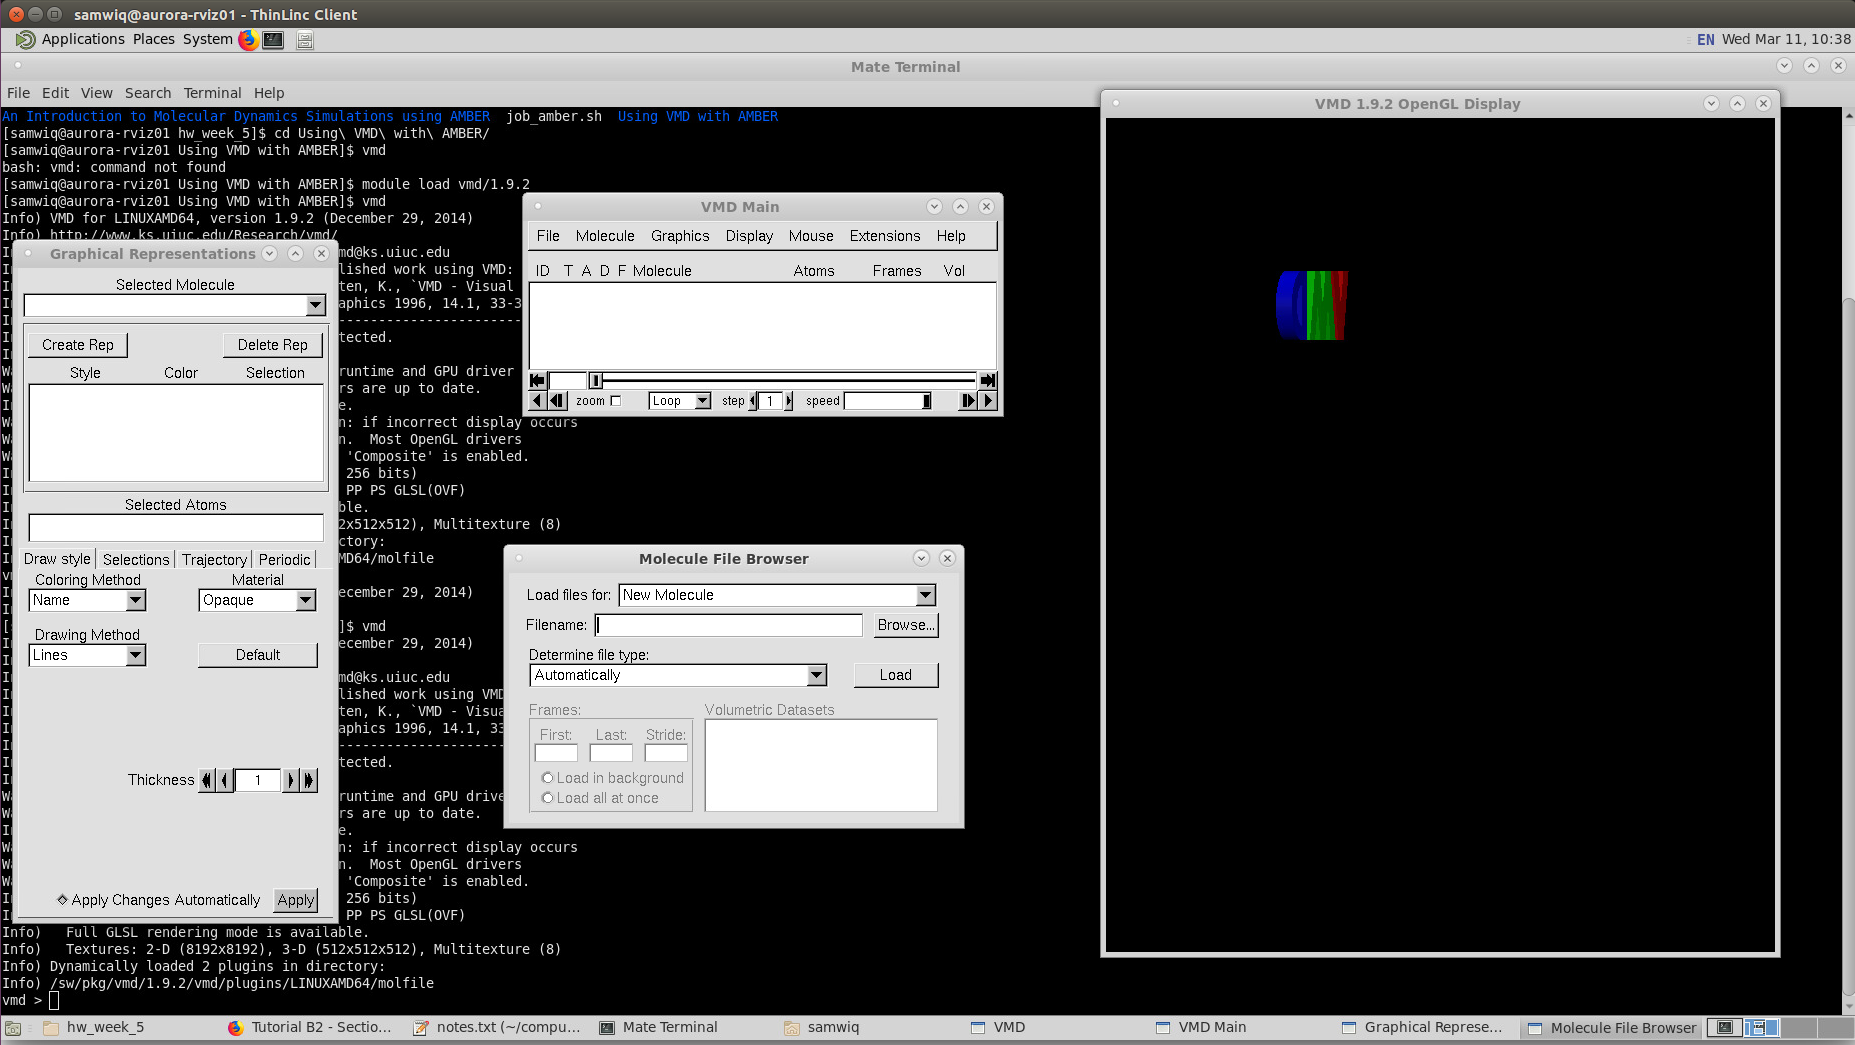
\includegraphics{Screenshot_vmd_setup.png}
\caption{VMD layout}
\end{figure}

\subsubsection{Section 2}\label{section-2}

The next step is to load the pde file of the Liver Alcohol Dehydrogenase
(LADH) molecule. After loading the file to VMD and testing out the
rotate, scale and translate of the OpenGl graphical interface we obtain
the following figure

\begin{figure}
\centering
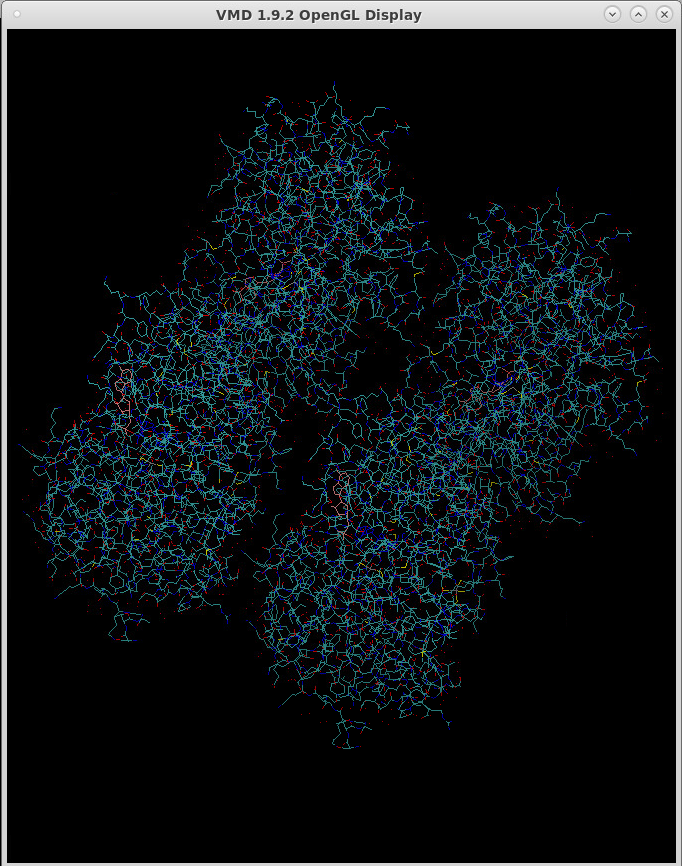
\includegraphics{Screenshot_ladh_in_opengl.png}
\caption{Shows the LAGH molecule in the OpenGL window}
\end{figure}

\subsubsection{Section 3}\label{section-3}

In this step, we used the graphical representation menu to change how to
display the LADH molecule. First, we removed all the water molecules
with the setting \texttt{all\ not\ water}; however, this didn't change
the visualization of the LADH molecule that much. Then we tried changing
the visualization by modifying the coloring method and the drawing
method. When using the coloring method \texttt{Secondary\ Structure} and
drawing method \texttt{NewCartoon} we obtained following visualization
of the LADH molecule

\begin{figure}
\centering
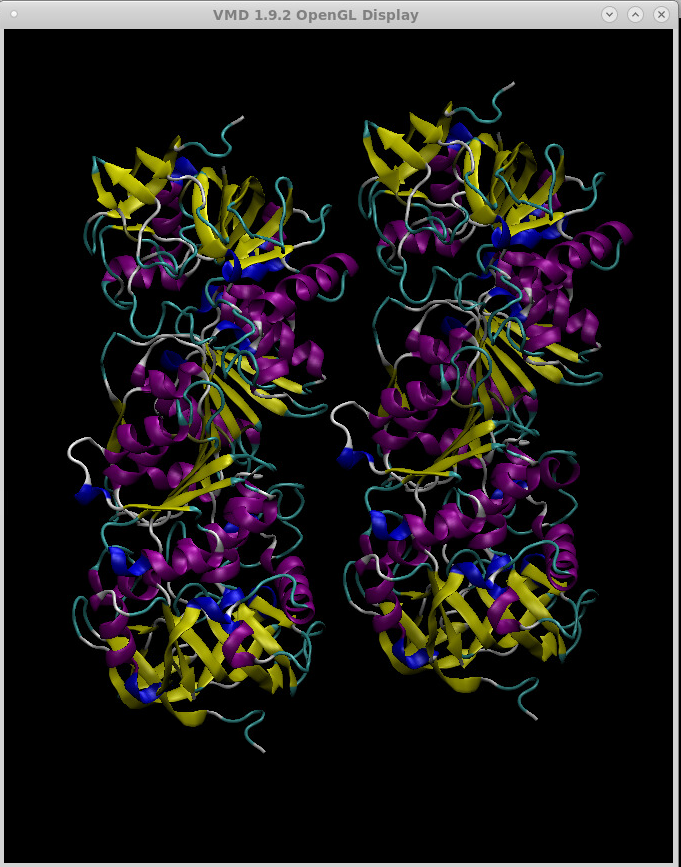
\includegraphics{Screenshot_ladh_new_vis.png}
\caption{Visualization using coloring method
\texttt{Secondary\ Structure} and drawing method \texttt{NewCartoon}}
\end{figure}

The last part of this section was to change the representation of the
molecule. When using the representation feature to only display the
chain A of the protine, we obtained the following visualization

\begin{figure}
\centering
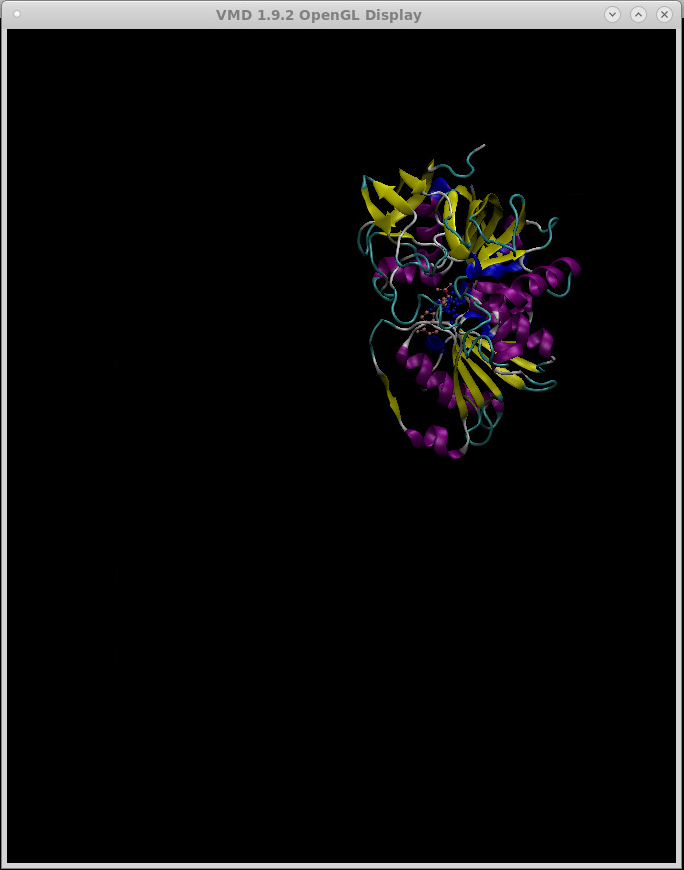
\includegraphics{Screenshot_ladh_only_chain_A.png}
\caption{Visualization displaying only chain A}
\end{figure}

\subsubsection{Section 4}\label{section-4}

First, we loaded the molecule stored in \texttt{TRPcage.pdb}, and then
after setting up the proper visulazation, we obtained the following
figure

\begin{figure}
\centering
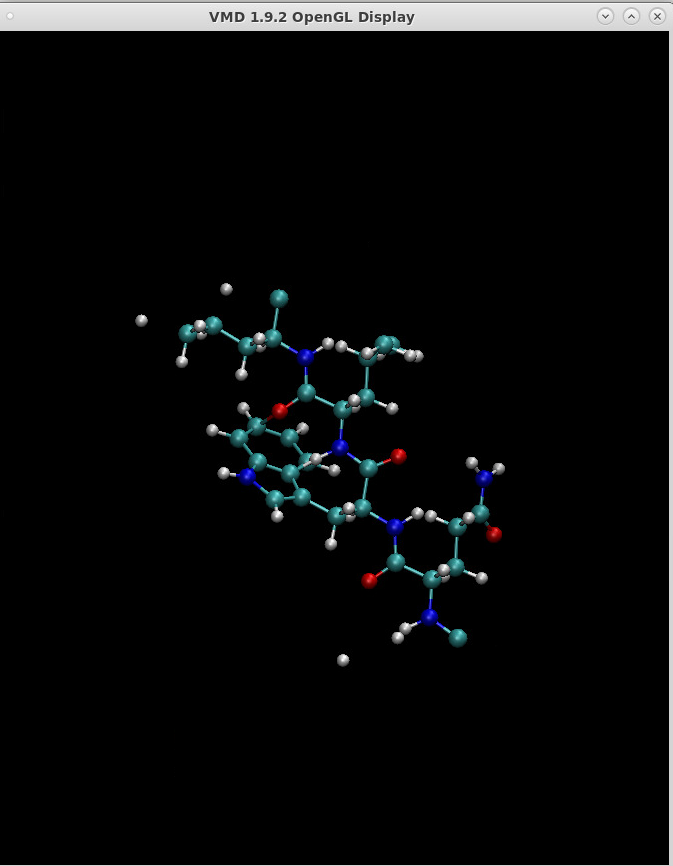
\includegraphics{Screenshot_first_fig_trp.png}
\caption{First Visualization of TRP}
\end{figure}

Then we loaded different versions of the molecule representing either
the minimized or unminimuizes structure: The minimized structure is
presented below

\begin{figure}
\centering
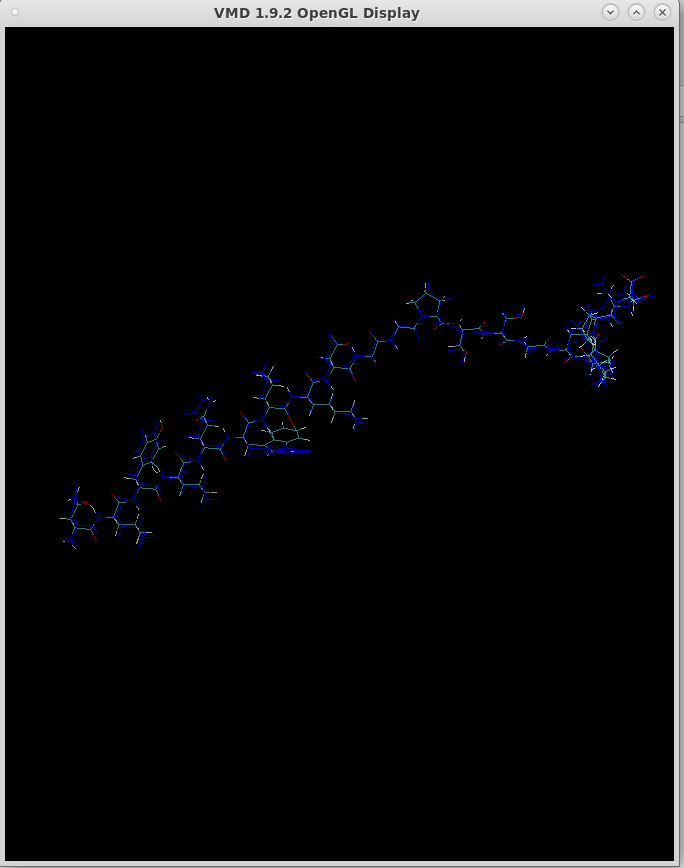
\includegraphics{Screenshot_fig_trp_min.png}
\caption{First Visualization of the minimized structure}
\end{figure}

\subsubsection{Section 5}\label{section-5}

In the first step of this section, we loaded two structures and fixed
one of them, so that we can rotate the other one without moving the
first one. For this task, we obtain the following figure

\begin{figure}
\centering
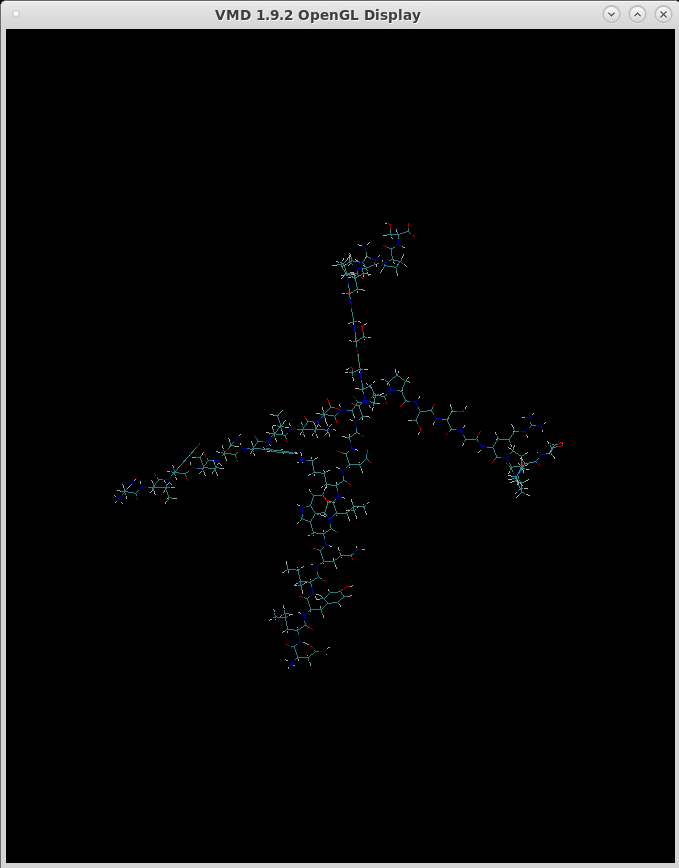
\includegraphics{Screenshot_rotate_one.png}
\caption{Figure of two molecules where we rotate one of the structures}
\end{figure}

The next step is to compute the RMSD between two structures where one of
the structures is a shifted version of the other. For this task, we
obtain RMSD to be \(\approx 2.18\) angstroms. We then aligned the
structures and again computed the RMSD. The RMSD between the aligned
structures was \(\approx 0.57\) angstroms. The aligned structures are
presented below.

\begin{figure}
\centering
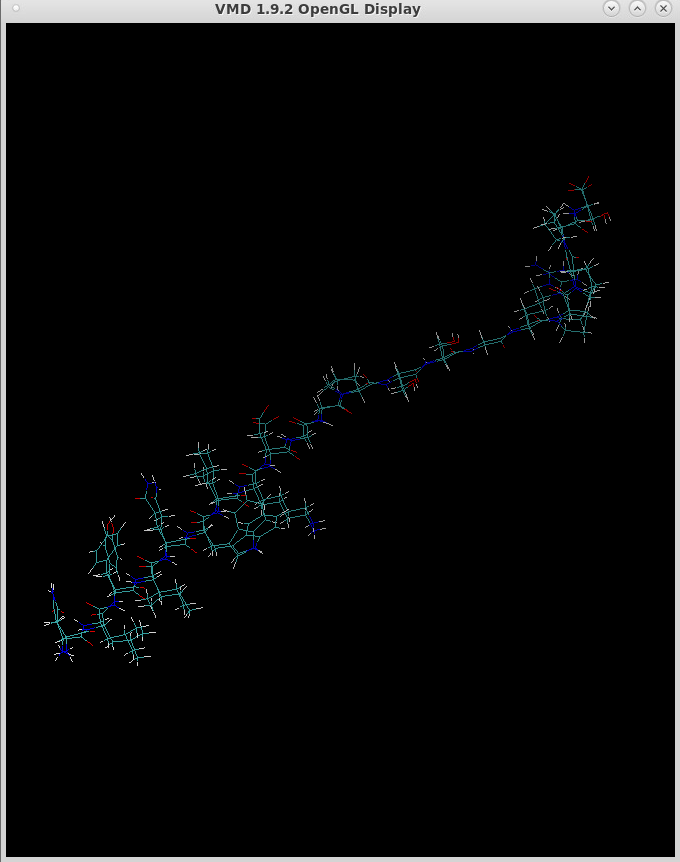
\includegraphics{Screenshot_algined.png}
\caption{The two aligned structures}
\end{figure}

\subsubsection{Section 6}\label{section-6}

In this task, we used VMD to visualize the trajectory path computed
using AMBER. The visualization and playback fo the structure during the
simulation worked well.

\subsubsection{Section 7}\label{section-7}

The task here was to save the simulation at frame 300 to a separate
\texttt{pdb} file. However, when we tried to do this, we got the error
message: \(Error writing trajectory file\). So we could not complete
this task. Instead, we downloaded the file we should have been able to
create from the tutorial web site.

\subsubsection{Section 8}\label{section-8}

In this task, we use the system parameter tracking capabilities to show
the distance between parts of the structure during the simulation. Frame
\(294\) of the simulation where we keep track of the distance between
the two ends of the structure is presented below

\begin{figure}
\centering
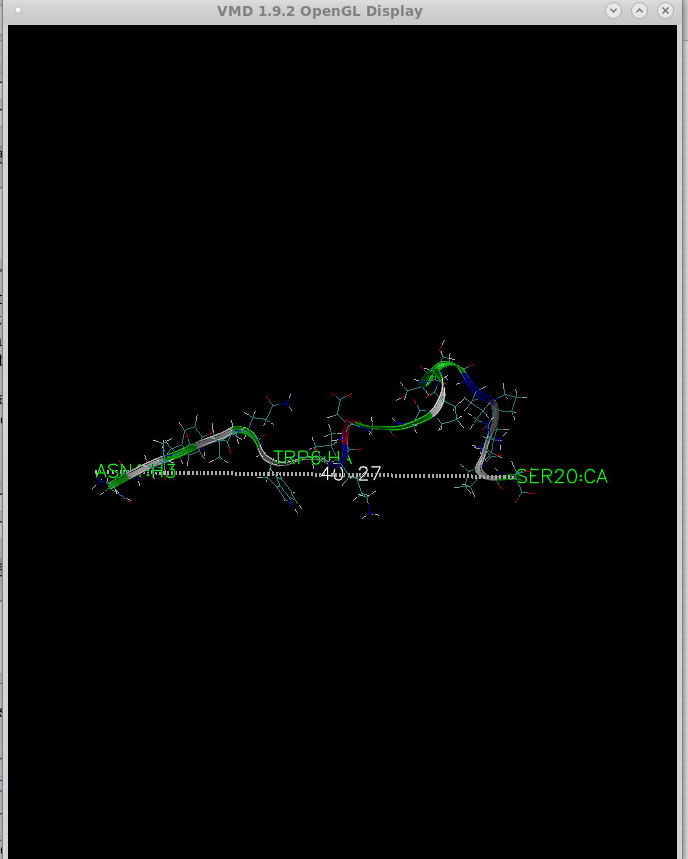
\includegraphics{Screenshot_dist_ends.png}
\caption{Frame 294 where we show the distance between he ends of the
structure}
\end{figure}

\subsubsection{Section 9}\label{section-9}

The final part included using VMD to create an \texttt{mpg} movie.
However, we could not create the movie since we got the error
\texttt{Program\ not\ found} saying that VMD could not locate
'ppmtompeg', when trying to create the movie.

    \section{Loop dynamics of the HIV-1 integrase core
domain}\label{loop-dynamics-of-the-hiv-1-integrase-core-domain}

The idea for this tutorial was to run an MD simulation. However, we
could not get the data setup to work, so we instead downloaded the files
from the webpage. The energy minimization and visualization tasks also
did not work properly, so we again downloaded the files from the webpage
and worked through the tutorial that way.

    \section{A case study in folding
Trp-Cage}\label{a-case-study-in-folding-trp-cage}

\subsubsection{Section 1}\label{section-1}

In this first section, we use \texttt{xleap} to create the structure
directly from the amino acid sequence. We present the sequence below
using the edit \texttt{command} in \texttt{xleap}

\begin{figure}
\centering
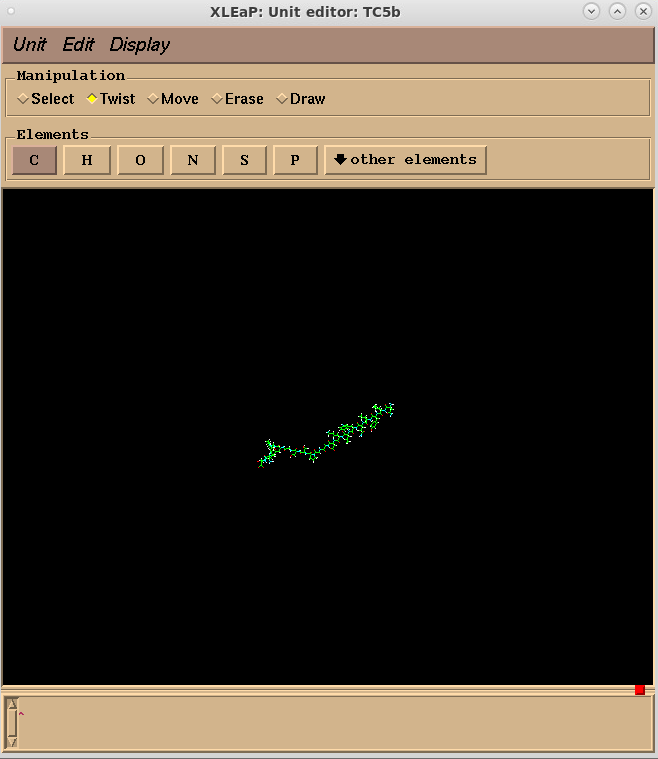
\includegraphics{Screenshot_xleap.png}
\caption{The sequence created in xleap}
\end{figure}

The final step here is to save the structure in a \texttt{lib} and
\texttt{pdb} file,

\subsubsection{Section 2}\label{section-2}

The task in this section was to load the Amber parameters of the
structure and save them in new files. This step worked well without any
problems.

\subsubsection{Section 3}\label{section-3}

In this section, we run the minimization in \texttt{AMBER} using the
input files we created in Section 1 and 2. The minimization ran without
any problems. After running the minimization, we used \texttt{VMD} to
view the final results, which are presented below. In \texttt{VMD} we
also compute the RMSD between the two structures, and the RMSD was
\(\approx 0.54\) angstrom.

\begin{figure}
\centering
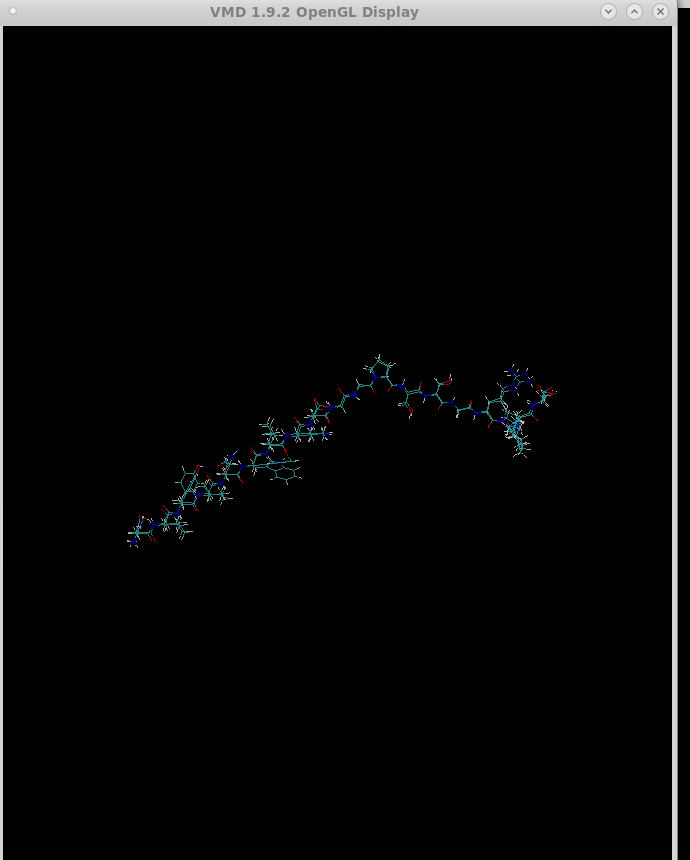
\includegraphics{Screenshot_input_and_final.png}
\caption{Comparing the input structure to the final minimized structure}
\end{figure}

\subsubsection{Section 4}\label{section-4}

I tried running the simulations for different heats with \texttt{AMBER}
using the following script

\begin{verbatim}
#!/bin/sh

# Set up for run:

# need this since I use a LU project
#SBATCH -A lu2019-2-19
#SBATCH -p lu


# use gpu nodes
#SBATCH -N 1
#SBATCH -n 1
# #SBATCH --mem-per-cpu=11000
# #SBATCH -C mem256GB

# time consumption HH:MM:SS
#SBATCH -t 1:00:00

# name for script
#SBATCH -J amber_run

# controll job outputs
#SBATCH -o outputs_amber_run_%j.out
#SBATCH -e errors_amber_run_%j.err

# notification
#SBATCH --mail-user=samuel.wiqvist@matstat.lu.se
#SBATCH --mail-type=ALL

# load modules
ml load  icc/2017.4.196-GCC-6.4.0-2.28
ml load OpenMPI/2.1.1
ml load Ambertools/18.10

mpirun -np 16 $AMBERHOME/bin/sander -O -i heat1.in -p TC5b.prmtop -c min1.ncrst -r heat1.ncrst -o heat1.out -x heat1.nc
gzip -9 heat1.nc
mpirun -np 16 $AMBERHOME/bin/sander -O -i heat2.in -p TC5b.prmtop -c heat1.ncrst -r heat2.ncrst -o heat2.out -x heat2.nc
gzip -9 heat2.nc
mpirun -np 16 $AMBERHOME/bin/sander -O -i heat3.in -p TC5b.prmtop -c heat2.ncrst -r heat3.ncrst -o heat3.out -x heat3.nc
gzip -9 heat3.nc
mpirun -np 16 $AMBERHOME/bin/sander -O -i heat4.in -p TC5b.prmtop -c heat3.ncrst -r heat4.ncrst -o heat4.out -x heat4.nc
gzip -9 heat4.nc
mpirun -np 16 $AMBERHOME/bin/sander -O -i heat5.in -p TC5b.prmtop -c heat4.ncrst -r heat5.ncrst -o heat5.out -x heat5.nc
gzip -9 heat5.nc
mpirun -np 16 $AMBERHOME/bin/sander -O -i heat6.in -p TC5b.prmtop -c heat5.ncrst -r heat6.ncrst -o heat6.out -x heat6.nc
gzip -9 heat6.nc
mpirun -np 16 $AMBERHOME/bin/sander -O -i heat7.in -p TC5b.prmtop -c heat6.ncrst -r heat7.ncrst -o heat7.out -x heat7.nc
gzip -9 heat7.nc
\end{verbatim}

However, this script failed, and we instead ran the simulations directly
on the local \texttt{LUNARC} node we used for the visualizations. After
running the simulations, the task was to use \texttt{VMD} to visualize
the simulations. But we could not get this step to work properly.

\subsubsection{Section 5}\label{section-5}

The task here was to run a long production run. However, I did not run
the production run but instead downloaded the results files from the
tutorial webpage. The next step was to visualize the simulations, but
the instructions for this step were very unclear, so we did not manage
to do that part.

\subsubsection{Section 6}\label{section-6}

In this section, we used \texttt{xmgrace} to visualize the summary
results, see figures below.

\begin{figure}
\centering
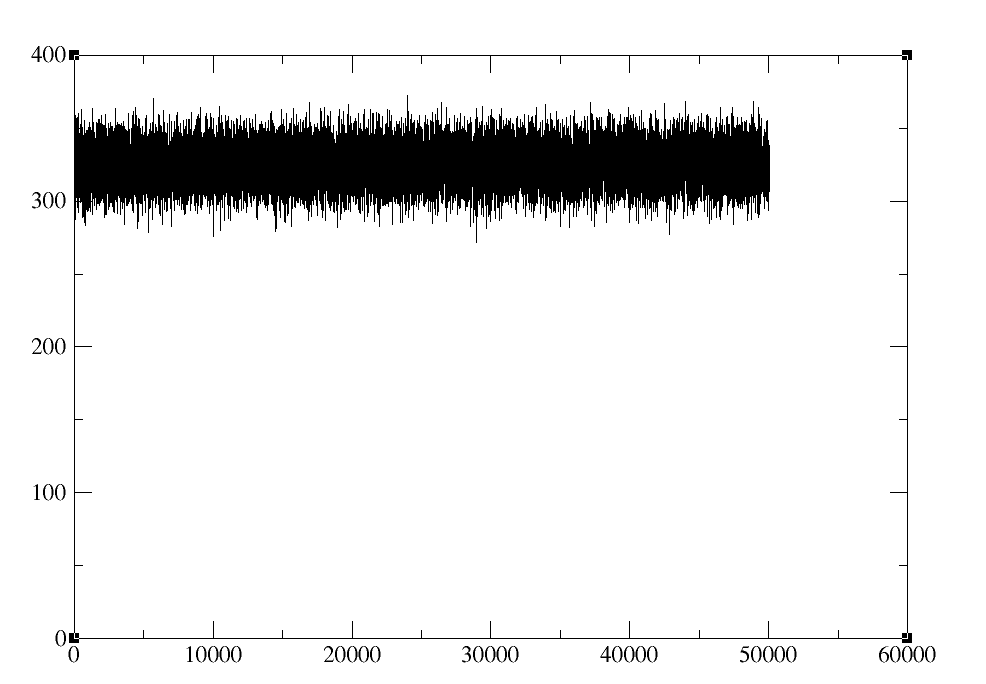
\includegraphics{Screenshot_temp.png}
\caption{Temprature}
\end{figure}

We also plot the Total Energy (Black), Potential Energy (Red), Kinetic
Energy (Green), see below

\begin{figure}
\centering
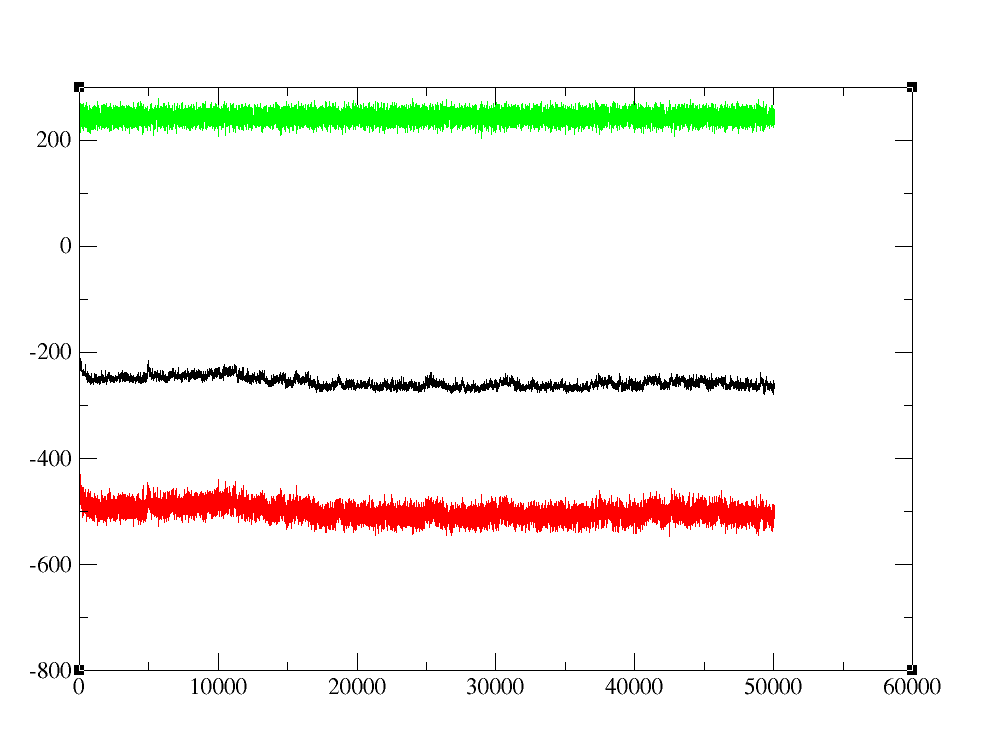
\includegraphics{Screenshot_energy.png}
\caption{Total Energy (Black), Potential Energy (Red), Kinetic Energy
(Green)}
\end{figure}

In this part, we also produced several other plots that we have not
included in this report.

\subsubsection{Section 7}\label{section-7}

For this section, the task was to redo the simulations for several other
settings and study the differences in results.

    \section{Thermodynamic Integration using soft core
potentials}\label{thermodynamic-integration-using-soft-core-potentials}

For this tutorial, we downloaded the files and scripts and worked
through the tutorial using the provided files and scripts.

    \section{Computing binding enthalpy
values}\label{computing-binding-enthalpy-values}

The first step was to use tleap to create the input files for the
simulations. Some of the tleap commands, however, failed, so we instead
downloaded the files from the tutorial webpage.

The next step was to run the minimization, but we could not get the
command \texttt{pmemd} to work (even after loading `AMBER), so we
instead downloaded the resulting files from the webpage.

For heating the system, we also restored to downloading the files from
the tutorial webpage.

Since we were not able to run the simulations, we also did not manage to
check the results, as suggested in the tutorial.

As suggested in the tutorial, we downloaded the result files from the
webpage instead of running the simulations. Of course, the results
(total energy numbers) that we calculated in section 4 were similar to
the ones on the webpage.

    \section{An Introduction to CPPTRAJ}\label{an-introduction-to-cpptraj}

We first tried to run a simple analysis using interactive mode, and
everything worked well. We then ran the same analysis using the batch
mode, and also that worked well.

\section{RMSD Analysis in CPPTRAJ}\label{rmsd-analysis-in-cpptraj}

In this tutorial, we ran a coordinate root-mean-squared deviation (RMSD)
analysis on the output from an MD simulation. We were not able to create
the plots (since it was not able to load both AMBER and Grace at the
same time), but this is a minor problem since the plots easily can be
created with many different plotting software or without first loading
AMBER.

In the second part of the tutorial, we used reference structures and
different topologies, and both these methods worked well.

\section{Hydrogen Bond Analysis with
CPPTRAJ}\label{hydrogen-bond-analysis-with-cpptraj}

In this tutorial, we used CPPTRAJ to find and track hydrogen bonds in a
molecule. We could run all analyses in this tutorial without problems.

    \section{Setting up and protonating with
Maestro}\label{setting-up-and-protonating-with-maestro}

The Maestro software was not installed on LUNARC, so we instead
installed the free version of Maestro on a local laptop.

After installing Maestro we tried to run the tutorial on lysozyme (PDE
181L: https://www.rcsb.org/structure/181L). However, some errors
occurred we tried to run the tutorial, so we did not manage to complete
it.


    % Add a bibliography block to the postdoc
    
    
    
    \end{document}
